\documentclass[11pt,a4paper]{article}

\usepackage[applemac]{inputenc}
\usepackage{latexsym}
\usepackage{graphicx}
\usepackage[english]{babel}
\usepackage{amsmath,amssymb}
\usepackage{pstricks,pst-plot}
\usepackage{calc}
\usepackage{multicol}
\usepackage{fancyhdr}
\usepackage{lastpage}
\usepackage[T1]{fontenc}
\usepackage{stmaryrd}
\usepackage{float}
\pagestyle{plain}



\begin{document}
	\title{Optimistic approaches in Contextual Linear Bandit models}
	\author{Mathurin \textsc{Massias} \and Clement \textsc{Nicolle}}
	\date{\today} 
	\maketitle
	
\subsection{LinUCB fir disjoint linear models}	

In the article \textit{A Contextual-Bandit Approach to Personalized News Article Recommendation}, the authors consider the case of a disjoint linear model, where we do not have $E[r_{t,a}|x_a] = x_{a}^T \theta^{*}$ anymore, but : $E[r_{t,a}|x_a] = x_{a}^T \theta_a^{*}$, i.e. a different $\theta$ for each possible arm. It is called "disjoint" as we do not have anymore the correlation between the arms.\\

Still, we wanted to study the differences with the previous linUCB algorithm. We now simulate a matrice $\theta$, and not a simple value, in which each column $a$ represents $\theta_a$.\\
In term of the algorithm, we add an initializing step. At the beginning, we need to pull each arm once, in order to have a first estimate of $\theta_a$ for each $a$ and a corresponding confidence interval.
Then, at iteration $t$, we pull the arm $a_t$ corresponding to $a_t = \mathrm{argmax}_{a_t} \widehat{\theta}_{a,t}^{T} x_a + \alpha \sqrt{x_a^T A_{a,t}^{-1} x_a}$ where $\widehat{\theta}_{a,t} = A_{a,t}^{-1}b_{a,t}$ is the estimate of $\theta_a$ at step $t$. In this sense, this algorithm can clearly be compared with UCB, unless we here try to fit a regression parameter.\\

The T-trial regret $R(T)$ can sill be written has $R(T) = E[\sum_{t=1}^{T} r_{t,a_t^{*}}] -  E[\sum_{t=1}^{T} r_{t,a_t}]$ where $a_t^{*}$ was the arm with the maximum expected reward among the pool of arms possible at step t.\\

For 1000 arms, we clearly see a high slope for the regret for the 1000 first iterations, corresponding to the initializing phase. As at each step we only have a more accurate estimate for a single $\theta_a$, the regret needs more time to decrease that in the case of LinUCB we saw before. Here, the regret is plotted for a horizon of 10 000 pulls of arms.

\begin{figure}[H]
	\centering
	\noindent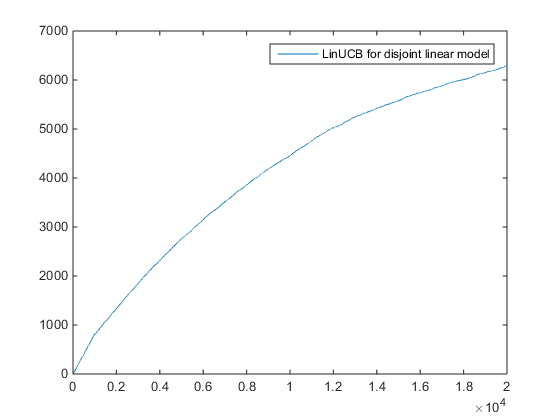
\includegraphics[scale=0.5]{regret-disjoint.png}
	\caption{Regret for disjoint linear model for 1000 arms, with 100 potentially arms pulled at each step, for $\sigma = 1$ at horizon 20 000}
\end{figure}

According to the article, this algorithm approaches a regret of $O(\sqrt{T})$.\\
By analyzing the arms pulled, we see that wheres the best arm had an expected reward of 0.7997, the most pulled arm had one of 0.7737, which is quite closed, and it was pulled 1094 times. The best potential arm was pulled 683 times.



\section{Comparison with Thompson Sampling}

\subsection{Thompson Sampling algorithm}

For Thompson Sampling algorithm, an assumption is made on the posterior distribution of $\theta$. Then, at each step $t$ we draw a sample $\widetilde{\theta}_t$ according to this distribution, and pull the arm $a_t$ corresponding to $a_{t} = \mathrm{argmax}_{a_t} \widetilde{\theta}_{t}^{T} x_a$.\\

The whole question is now : what model should we take for the posterior probability ? In her thesis, Emilie Kaufmann proposes to take a Gaussian law. Indeed, with a noise $\eta_t \sim \mathcal{N}(0,\sigma^2)$, we can draw $\widetilde{\theta}_{t}$ according to the law $\mathcal{N}(\widehat{\theta}_t,v_t^2 A_t^{-1})$ where $\widehat{\theta}_t = A_{t}^{-1}b_{t}$ is the estimate of $\theta$ at step $t$,  $v_t = \sigma \sqrt{9 d log \frac{t}{\delta}}$ and $A_t = I_d + X_{1:t}X_{1:t}^T$, to obtain a confidence interval with probability at least $1-\delta$ in dimension $d$.

\subsection{Results}

With Thompson Sampling, we clearly see the impact of the noise and its variance $\sigma^2$. Indeed, here is the regret achieved for different values of $\sigma^2$.

\begin{figure}[H]
	\centering
	\noindent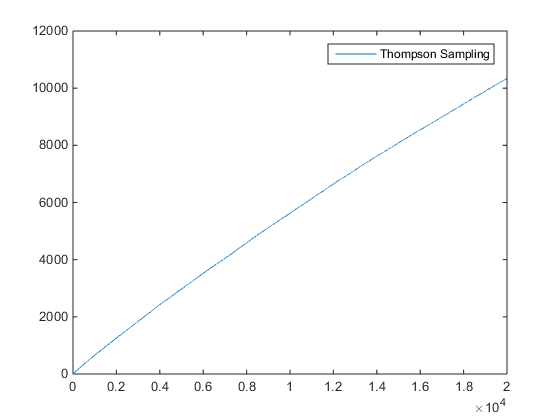
\includegraphics[scale=0.25]{thompson_noise1.png}
	\noindent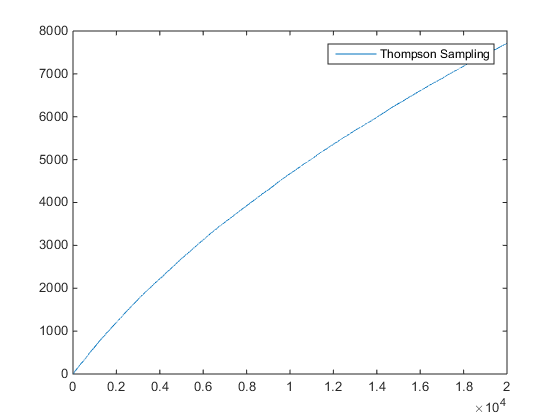
\includegraphics[scale=0.25]{thompson_noise05.png}
	\noindent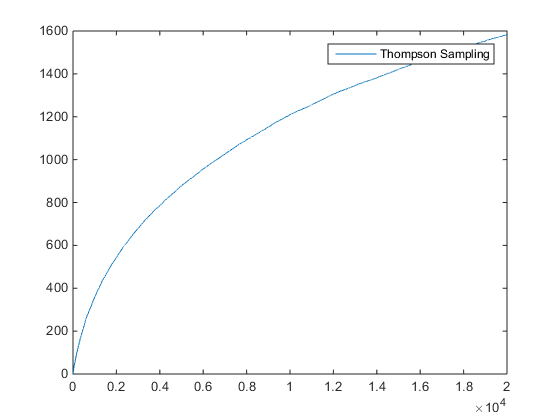
\includegraphics[scale=0.25]{thompson_noise01.png}
	\caption{Left : regret for Thompson Sampling with $\sigma^2 = 1$ - Middle : $sigma^2 = 0.5$ - Right : $sigma^2 = 0.1$}
\end{figure}

For  $\sigma^2 = 0.1$, the best arm was effectively the most pulled, and it was pulled 1549 times over 20 000. But for $\sigma^2 = 1$, the most pulled arm was only pulled 83 times, for an expected regret of 0.7433 to be compared with 0.8377 for the best arm. We see that the algorithm is much less accurate for high value of $\sigma^2 = 0.1$, which seems logical, as we draw $\widehat{\theta}_t$ according to a normal law whose variance directly depends on $\sigma$. 


\end{document}